% Options for packages loaded elsewhere
\PassOptionsToPackage{unicode}{hyperref}
\PassOptionsToPackage{hyphens}{url}
%
\documentclass[
  man,floatsintext,
  man]{apa6}

\usepackage{amsmath}
\usepackage{amsthm}
\usepackage{framed}
\usepackage{pifont}
\usepackage{listings}
\usepackage{tikz}
\usepackage{hyperref}
\usepackage{float}
\usepackage{paralist}
\usepackage{xcolor}
\usepackage{tikz}
\usepackage{siunitx}
\usepackage{float}
\newenvironment{smalltable}{\begin{table}[H]\footnotesize}{\end{table}}
\usepackage{hanging}
\ifLuaTeX
  \usepackage{selnolig}  % disable illegal ligatures
\fi
\usepackage[]{biblatex}
\addbibresource{r-references.bib}
\IfFileExists{bookmark.sty}{\usepackage{bookmark}}{\usepackage{hyperref}}
\IfFileExists{xurl.sty}{\usepackage{xurl}}{} % add URL line breaks if available
\urlstyle{same}
\hypersetup{
  pdftitle={Discover the Influence of Econmic Variables on CPI},
  pdfauthor={Ruiming Min1, Zicheng Wang2, Qi Yang3, \& Shumeng Zhang4},
  pdflang={en-EN},
  hidelinks,
  pdfcreator={LaTeX via pandoc}}

\title{Discover the Influence of Econmic Variables on CPI}
\author{Ruiming Min\textsuperscript{1}, Zicheng Wang\textsuperscript{2}, Qi Yang\textsuperscript{3}, \& Shumeng Zhang\textsuperscript{4}}
\date{}


\shorttitle{CPI and the Economic Variables}

\authornote{

NetIDs
RuiMing Min:rmin4
Zicheng Wang:zw70
Qi Yang:qiy4
Shumeng Zhang:sz65

The authors made the following contributions. Ruiming Min: Conceptualization, Data curation, Resources, Formal Analysis, Methodology, Writing - Original Draft Preparation, Writing - Review \& Editing; Zicheng Wang: Writing - Discussion, phrase, grammar, Final review and provide suggestions, Writing - Citation and Reference management; Qi Yang: Writing - Abstract \& Result comment \& report, Writing - Review \& Editing; Shumeng Zhang: Writing - Introduction, Writing - Review \& Editing.

}

\affiliation{\vspace{0.5cm}\textsuperscript{5} UIUC}

\abstract{%
This study employs time series analysis to investigate the Consumer Price Index (CPI), a crucial economic indicator reflecting changes in the average price level of goods and services. The main result reveals that incorporating economic variables, including the unemployment rate, real consumption, real government spending, and real investment, significantly enhances the prediction of CPI in the time series analysis model. The main result further confirms that positive coefficients for real consumption, real government spending, and real investment while negative for the unemployment rate indicate that these factors contribute to CPI growth aligning with economic theory. The CPI model's statistical significance, accuracy in fitting historical data, and precision in forecasting CPI values highlight the influential role of economic variables in shaping the CPI. This study provides valuable insights into the relationship between economic variables and CPI that may contribute to future research in an economic-related field, and provides an interpretable way of capturing CPI.
}



\begin{document}
\maketitle

\section{Introduction}\label{introduction}

Economics is a highly applicable field for the utilization of time series analysis. The volume of data is abundant and inherently indexed with time. By using the time series statistical models, we can leverage historical data to catch trends and patterns for the data and make reasonable predictions.

\subsection{Consumer Price Index (CPI)}\label{consumer-price-index-cpi}

In this project, we are analyzing the Consumer Price Index (CPI), a widely-used economic indicator that measures changes in the average price level of a basket of goods in an economic entity. It is commonly used to track inflation and assess price changes. A positive CPI value indicates inflation, while a negative value indicates deflation in the market. The goods' prices selected to calculate this index typically represent the overall prices of goods and services in society.
CPI is calculated relative to the price in the previous time period, which is assigned a value of 100. The percentage difference between the current price and the previous price is reflected in the index using a weighted average formula. Generally, a CPI increase of 3\% is considered inflation, while values over 5\% may indicate significant inflation in the economic entity. There are also some variants of CPI. Such as core CPI which excludes volatile food and energy prices, and regional CPIs, which focus on CPI values in specific geographical areas.
Given the critical role CPI plays in the economic landscape, we will introduce our approach to explore temporal and seasonal data patterns of CPI.

\subsection{Related Research}\label{related-research}

One of the seminal papers in this field is by James H. Stock(Stock,2019). His research primarily centers around the Phillips curve, which describes the connection between inflation and the unemployment rate. In our own research, employment stands out as a crucial metric that we analyze.
In recent years, there has been some research employing machine learning and deep neural networks for the prediction(Nguyen,2023;Barkan,2023). These models have strong performance, particularly with large datasets and when forecasting extended timeframes. However, it is important to note that due to the nature of these complex machine learning models, they often lack interpretability or the ability to provide clear explanations for their predictions.

\subsection{Data Sources and Analysis Approach}\label{data-sources-and-analysis-approach}

Our primary data sources include critical economic indicators, including the unemployment rate, government expenditure, investment, and consumption. These indicators play a pivotal role in measuring the level of economic activity within the entity. Furthermore, in our analytical approach, we use lagged and transformed Consumer Purchasing Index values, in conjunction with time-related variables, to enrich the comprehensiveness and precision of our assessments. It's worth noting that all these data elements are aligned with our response variable and are collected on a monthly basis.

\section{Methods}\label{methods}

To address the problem at hand, we used the following three steps to analyze the data: 1. detrending, 2. adding the economic variables, 3. lag analysis.

\subsection{Detrending}\label{detrending}

Observing the original data, the CPI has a significantly exponential trend. So we first use an exponential model to fit the data.
Moreover, according to the nature of the CPI, which is highly related to the inflation rate, and the average inflation rate, we choose 1.05 as the base of the exponential model.

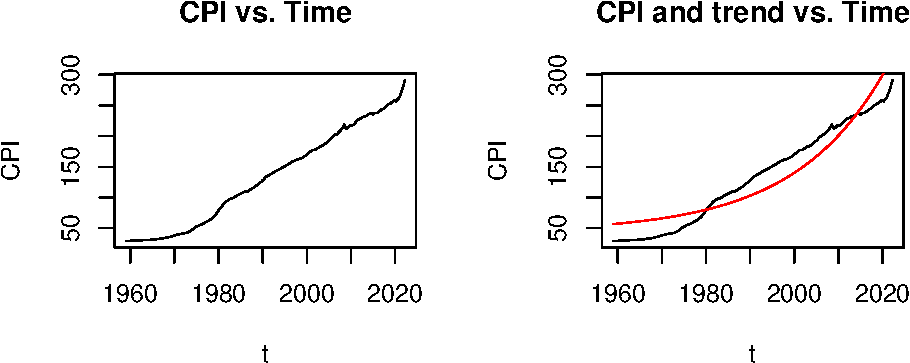
\includegraphics{stat429_group2_final_proj_files/figure-latex/unnamed-chunk-1-1.pdf}

\subsection{Adding the economic variables}\label{adding-the-economic-variables}

After the detrending, the time series of CPI, \(\{CPI(t)\}\), has become \(CPI(t) = T(t) + Y_t\).

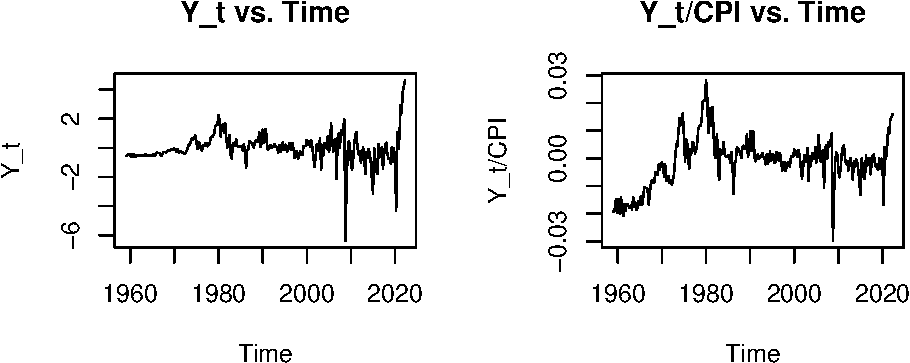
\includegraphics{stat429_group2_final_proj_files/figure-latex/unnamed-chunk-2-1.pdf}

The plot above shows that \(Y_t\) still does not behave like a white noise.
Additionally, the significant depressions in 2008 and 2020 and the significant peak in 1979 reflected the influence of the economic crisis(Gross,2019;Williams,2010:Barone,2019).
So we add some economic variables to the model to regress the final model.
Also, we add the sine functions of time to the model to fit the seasonal effect of the business cycle.

According to the nature of CPI(Blanchard,2004), \(CPI(t) = \frac{\sum_{i \in \mathcal{P}} P_{i,t} Q_i}{\sum_{i \in \mathcal{P}} P_{i,0} Q_i}\), where \(\mathcal{P}\) is the set of all goods and services, \(P_{i,t}\) is the price of good or service \(i\) at time \(t\), and \(Q_i\) is the quantity of good or service \(i\) at the base period.
Since the Wage-Setting Relation, \(W = \mathcal{A} P^e F(u,z)\), where \(W\) is the nominal wage, \(\mathcal{A}\) is the price mark-up, \(F(u,z)\) is the function of unemployment rate and other variables, \(u\) is the unemployment rate, and z is the output(GDP), and the Price-Setting Relation, \(P = (1+m)\frac{W}{\mathcal{A}}\), where \(m\) is the desired mark-up,
it is concluded as
\[CPI(t) = \frac{\sum_{i \in \mathcal{P}} (1+m_i) \frac{W_i}{\mathcal{A}} Q_i}{\sum_{i \in \mathcal{P}} P_{i,0} Q_i} = \frac{\sum_{i \in \mathcal{P}} (1+m_i) P_{i,t}^e F(u,z) Q_i}{\sum_{i \in \mathcal{P}} P_{i,0} Q_i}\].

To simplify the formula, we assume \(m_i = m \,\, \forall i\) and \(P_{i,t}^e = P_{i,t-1}\), we get \(CPI(t) = CPI(t-1) (1+m) F(u,z)\).
By the assumption of \(m\) is small and \(F(u,z) = 1 - \alpha u + \beta z\), we get \(CPI(t) = CPI(t-1) (1+m) (1 - \alpha u + \beta z)\) \(\cong CPI(t-1) ( 1 + m - \alpha u - \beta z)\).
We could conclude \(CPI(t)=CPI(t-1)(1 + m - \alpha u + \beta z)\).
For easy-computation, we assume CPI(t-1) is a constant we get \(CPI(t)=CPI_0(1 + m - \alpha u + \beta z)\).
Therefore we add the unemployment rate, the real consumption, real government spending, and the real investment to the model.

Moreover, we add the sine functions of time to the model to fit the seasonal effect of the business cycle and the square of time to fit the trend of the CPI.

To summarize the first model, we get the model as follows:

\begin{align*}
CPI(t) =& a_0 + a_1 \cdot 1.05^t  + a_2 (t-1959)^2 && (\text{trend})\\
& + a_3 \sin\left(\frac{2\pi(t-1959)}{40}\right) + a_4 \sin\left(\frac{2\pi(t-1980)}{24}\right) + && (\text{business cycle})\\
& + b_1 C_t + b_2 u_t + b_3 G_t + b_4 I_t + W_t && (\text{economic variables})
\end{align*}

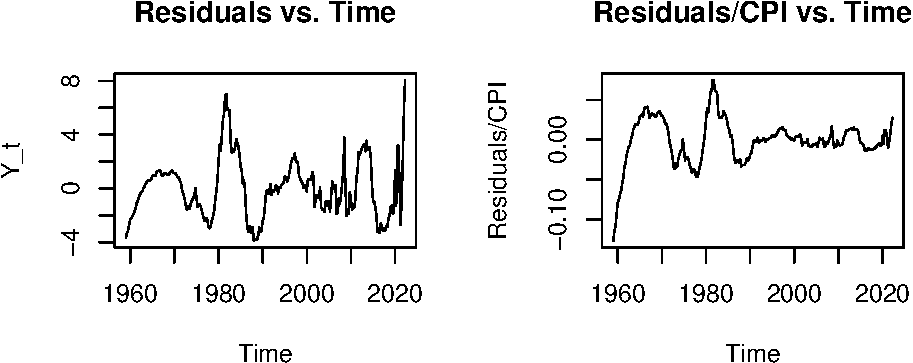
\includegraphics{stat429_group2_final_proj_files/figure-latex/unnamed-chunk-3-1.pdf}

The plot above shows that residuals still dose not behave like a white noise.
Therefore, we will use ACF to figure out weather or not the data has lags and improve our model.

\subsection{Lag Analysis}\label{lag-analysis}

After concluding the first model, we use PACF to figure out weather or not the data has lags.
From the plot below, the data has one lags.
Therefore, the CPI may be a AR(1) process
and we improve our model by adding the first order lag of CPI to the model.

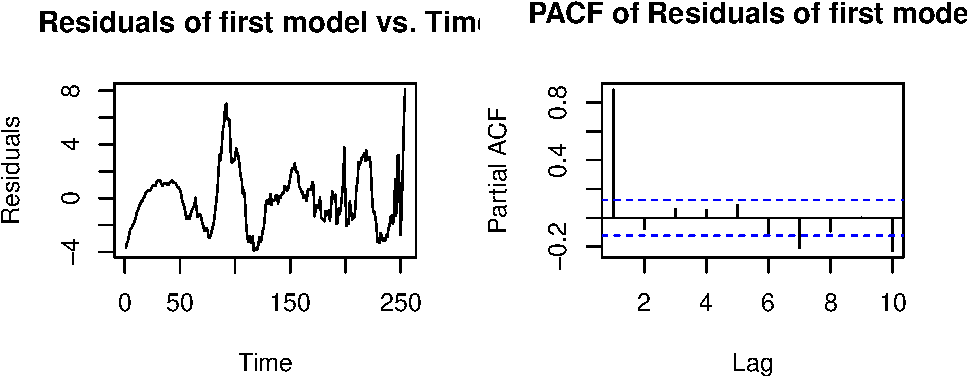
\includegraphics{stat429_group2_final_proj_files/figure-latex/unnamed-chunk-4-1.pdf}

Moreover, we delete the square of time from the model since it is not significant.

To summarize the second model, we get the final model as follows:

\begin{align*}
CPI(t) =& a_0 + a_1 \cdot 1.05^t + a_2 CPI(t-1)  && (\text{trend and lags})\\
& + a_3 \sin\left(\frac{2\pi(t-1959)}{40}\right) + a_4 \sin\left(\frac{2\pi(t-1980)}{24}\right) + a_5 \sin\left(\frac{2\pi(t-1980)}{48}\right)  && (\text{business cycle})\\
& + b_1 C_t + b_2 u_t + b_3 G_t + b_4 I_t + W_t && (\text{economic variables})
\end{align*}

where \(W_t\) is a white noise.

\section{Results}\label{results}

\subsection{Fitting Results}\label{fitting-results}

The fitted result of the model is shown below.

\bgroup \begin{table}[H]\footnotesize
    \centering
    \begin{tabular}{
      l
      S
      S[table-format=3.4]
      S[table-format=2.3]
      S[table-format=1.4e-2]
    }
    \toprule
    {Coefficients} & {Estimate} & {Std. Error} & {t value} & {Pr(>|t|)}  \\
    \midrule
(Intercept) & 2.159e+00 & 4.662e-01 & 4.632 & 5.90e-06  \\
I(1.05\textasciicircum t) & -8.779e-42 & 1.245e-42 & -7.050 & 1.83e-11\\
sin\_1 & -3.881e+00 & 6.540e-01 & -5.934 & 1.01e-08\\
sin\_2 & -1.028e+00 & 1.593e-01 & -6.455 & 5.80e-10 \\
sin\_3 & -3.760e+00 & 9.484e-01 & -3.965 & 9.66e-05  \\
CPI\_lag1 & 9.735e-01 & 1.351e-02 & 72.033 & < 2e-16  \\
unemp\_rate & 1.847e-01 & 5.406e-02 & 3.416 & 0.000745  \\
grove\_exp & 6.250e-04 & 2.178e-04 & 2.870 & 0.004470  \\
invest & 7.797e-04 & 3.737e-04 & 2.087 & 0.037966  \\
consump\_real & 3.423e-03 & 3.337e-04 & 10.259 & < 2e-16 \\
    \bottomrule
\end{tabular}
\end{table}\egroup

\[
\begin{aligned}
&\text{Residual standard error: 0.8011 on 244 degrees of freedom} \\
&\text{Multiple R-squared: 0.9999, Adjusted R-squared: 0.9999} \\
&\text{F-statistic: 2.688e+05 on 9 and 244 DF, p-value: < 2.2e-16}
\end{aligned}
\]

After we add the selected economic variables including the unemployment rate, real consumption, real government spending, and real investment to the model. We generate an overall table above to examine the fit of the variables. From the table above, we can find out all the added economic variables have p-values 0.000745 for the unemployment rate,\(<2 \times 10^{-16}\) for real consumption, 0.004470 for real government pending,0.037966 for real investment, therefore, we can conclude that all the added economic variables in the table are statistically significant. For the entire model, we can find out the R squared is 0.9999 which is large enough to conclude that the added economic variables fit the data well, and the p-value for the F test is less than \(\alpha\)(0.05), therefore, we can conclude that the model is statistically significant. Based on the result above, we can conclude that CPI will be influenced by the unemployment rate, real consumption, real government spending, and real investment.

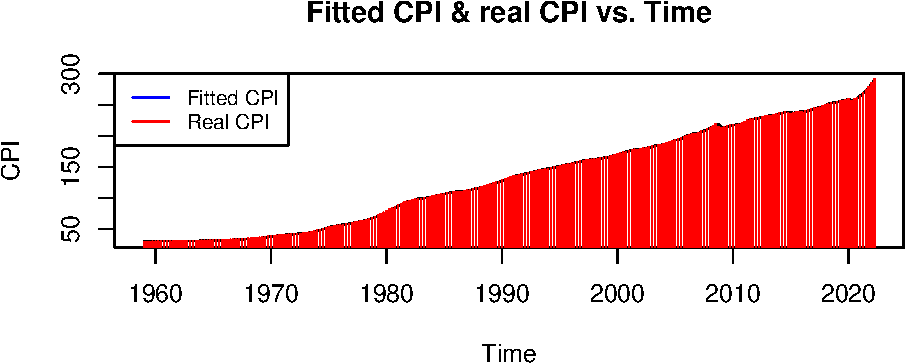
\includegraphics{stat429_group2_final_proj_files/figure-latex/unnamed-chunk-5-1.pdf}

The graph above is the comparison between our model after adding the economic variables and the real CPI versus the time that we can find in the data. The model seems to completely fit with the real CPI. Therefore, the graph further confirms our research and the added economic variables are essential for fitting a CPI model to contribute significantly to the model's precision.

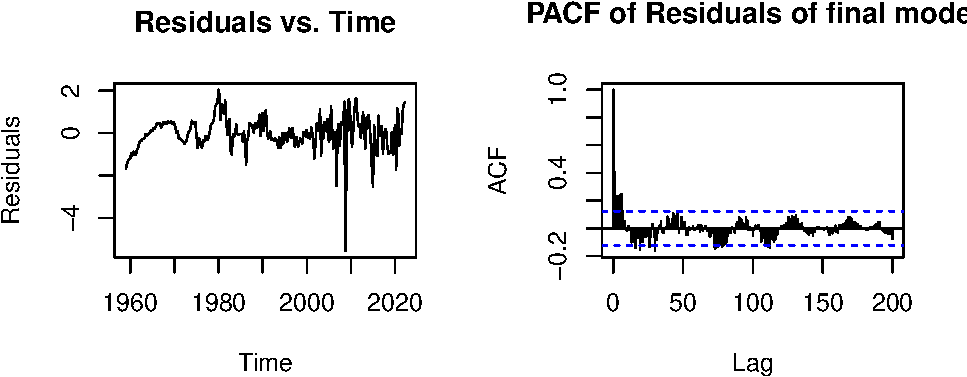
\includegraphics{stat429_group2_final_proj_files/figure-latex/unnamed-chunk-6-1.pdf}

To check our model, we perform an analysis of residuals to ensure that the CPI model's predictions are unbiased. We can find out the overall residuals plot shows the difference between predicted CPI values and the real CPI against time. Although a depression in 2010 and a relatively upward trend the 1960 to 1970 is noticeable, the residuals overall resemble white noise at other points, indicating a better fit of the model(Bryan,2013). The reason for the upward trend from 1960 to 1970 may be because of the robust consumer spending after World War II, the low unemployment rate, and Vietnam War spending. All these factors are included in the economic variables added to the model, therefore, these may be the reason for the upward trend. Also, for the noticeable depression before 2010, the reason may be the financial crisis in 2008(Blinder,2015). These are the cases that are worth the discussion in the future. Additionally, the autocorrelation function (ACF) plot demonstrates that the correlations of residuals largely fall within the confidence interval, affirming the CPI model is significant.

\subsection{Forecasting Results}\label{forecasting-results}

The forecasting result of the model is shown below. The analysis of the percentage prediction errors over time reveals a promising performance of the model in predicting the CPI. The plot illustrates that the errors are consistently small across the entire time range, with the majority of the percentage errors approximately around zero. This indicates a remarkable alignment between the predicted CPI values and the actual CPI values during the test period. Furthermore, the mean squared error is \(7.185918 \times 10^{-5}\) which confirms the model's precision. The small errors and low mean squared error suggest that the model has effectively captured the CPI data, showing its reliability in forecasting future CPI values. , the prediction is also a confirmation of the importance of the added economic variables the unemployment rate, real consumption, real government spending, and real investment in the model.

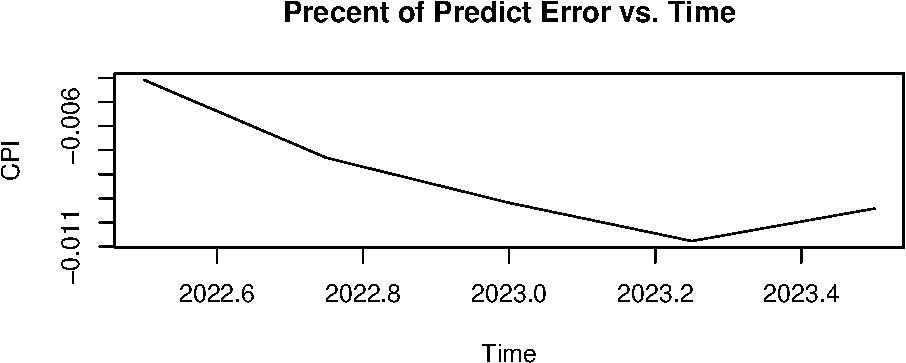
\includegraphics{stat429_group2_final_proj_files/figure-latex/unnamed-chunk-7-1.pdf}

In conclusion, the model's statistical significance, accuracy in fitting historical data, and precision in forecasting CPI values highlight the influential role of economic variables in shaping the CPI. The positive coefficient estimates for real consumption, real government spending, and real investment indicate that an increase in these variables is associated with a rise in the CPI. This aligns with standard economic theory, where increased consumer spending, government expenditure, and investment often contribute to overall economic growth and can lead to higher inflation.Conversely, the negative coefficient estimate for the unemployment rate suggests an inverse relationship with the CPI. Higher unemployment rates tend to be associated with economic downturns, leading to decreased consumer spending and overall demand, which can put downward pressure on prices and inflation. As the analysis encompasses both statistical and practical significance, these findings contribute valuable insights for understanding the relationship between economic variables and the CPI, providing insights for investigation further.

\section{Discussion}\label{discussion}

\subsection{Main summary of the current study}\label{main-summary-of-the-current-study}

By running a time series analysis on incorporated economic variables: unemployment rate, real consumption, real government spending, and real investment, it is evidently shown these economic variables are significant in predicting CPI. The model developed in this study to predict (Consumer Price Index)CPI is:

\begin{align*}
CPI(t) =& a_0 + a_1 \cdot 1.05^t + a_2 CPI(t-1)  && (\text{trend and lags})\\
& + a_3 \sin\left(\frac{2\pi(t-1959)}{40}\right) + a_4 \sin\left(\frac{2\pi(t-1980)}{24}\right) + a_5 \sin\left(\frac{2\pi(t-1980)}{48}\right) && (\text{business cycle})\\
& + b_1 C_t + b_2 u_t + b_3 G_t + b_4 I_t + W_t && (\text{economic variables})
\end{align*}
shows great accuracy in predicting CPI. This achieves the goal described above of finding a pattern of CPI, also the model provides clear interpretability by finding the most suitable coefficients, inspired and derived from economic theories for the model.

\subsection{Other famous research or academic outcomes}\label{other-famous-research-or-academic-outcomes}

The model concluded by this study aligns with Keynesian economic theory(Corry,1986), which also concludes that government spending, unemployment, and other common factors play an important role in economic performance, reflected in inflation. The Milton Friedman's Monetarist critique also indicates the positive relationship between real consumption and inflation rate(Vaggi,2003). The conclusions of these two theories are consistent with the findings of this study.

\subsection{Flaws in the current study}\label{flaws-in-the-current-study}

The study lacks investigation into other common factors influencing CPI. For example, international trade dynamics or other economic unexpected events. The main method this study uses to conduct statistical analysis is time series analysis. However, it is possible the evolving economic factors' own nature overlooks the factor of time, resulting in an inappropriate method of conducting an investigation due to the evolving nature of economic factors. Another possible issue is the near-perfect R-squared value, which could possibly indicate the sign of overfitting, indicating a lack of generalization of unseen data.

\subsection{Suggestions on future, additional future.}\label{suggestions-on-future-additional-future.}

The major suggestion is to continue investigating other economic factors, like international trade dynamics, and exchange rates, to have a deeper insight into how economic factors impact CPI. Based on the near-perfect R-squared value of this study, the model could apply regularization techniques to detect and prevent the problem of overfitting. By the nature of economic variables, the future study could take a deeper look into some unexpected events and apply the developed model, too, which could validate the model's effectiveness. These suggestions will help build a more solid understanding of CPI.

\newpage

\section{References}\label{references}

\begin{hangparas}{4em}{1}
\noindent Barkan, O., Benchimol, J., Caspi, I., Cohen, E., Hammer, A., \& Koenigstein, N. (2023). Forecasting CPI inflation components with Hierarchical Recurrent Neural Networks. International Journal of Forecasting, 39(3), 1145-1162. https://doi.org/10.1016/j.ijforecast.2022.04.009 \newline
\end{hangparas}

\begin{hangparas}{4em}{1}
\noindent Barone, R. (2019). A Strange New World: Economic Slowdown, Liquidity Issues. Retrieved from https://www.forbes.com/sites/greatspeculations/2019/09/22/a-strange-new-world-economic-slowdown-liquidity-issues/?sh=4b97f34b89ff \newline
\end{hangparas}

\begin{hangparas}{4em}{1}
\noindent Blanchard, O. J., \& Sheen, J. R. (2004). Macroeconomics. Pearson Education.\newline
\end{hangparas}

\begin{hangparas}{4em}{1}
\noindent Blinder, A. S., \& Zandi, M. (2015). The Financial Crisis: Lessons for the Next One. Retrieved from https://www.cbpp.org/research/the-financial-crisis-lessons-for-the-next-one \newline
\end{hangparas}

\begin{hangparas}{4em}{1}
\noindent Bryan, M. (2013). The Great Inflation. Retrieved from https://www.federalreservehistory.org/essays/great-inflation \newline
\end{hangparas}

\begin{hangparas}{4em}{1}
\noindent Corry, B. (1986). Keynes's Economics: A Revolution in Economic Theory or in Economic Policy? In R. D. Collison Black (Ed.), Keynes's Economics. Palgrave Macmillan UK.\newline
\end{hangparas}

\begin{hangparas}{4em}{1}
\noindent Gross, S. (2019). What Iran's 1979 revolution meant for US and global oil markets. Retrieved March 2019, from https://www.brookings.edu/articles/what-irans-1979-revolution-meant-for-us-and-global-oil-markets/ \newline
\end{hangparas}

\begin{hangparas}{4em}{1}
\noindent Nguyen, T.-T., Nguyen, H.-G., Lee, J.-Y., Wang, Y.-L., \& Tsai, C.-S. (2023). The consumer price index prediction using machine learning approaches: Evidence from the United States. Heliyon, 9(10), Article e20730. https://doi.org/10.1016/j.heliyon.2023.e20730 \newline
\end{hangparas}

\begin{hangparas}{4em}{1}
\noindent Stock, J. H., \& Watson, M. W. (1999). Forecasting inflation. Journal of Monetary Economics, 44(2), 293-335. https://doi.org/10.1016/S0304-3932(99)00027-6 \newline
\end{hangparas}

\begin{hangparas}{4em}{1}
\noindent Vaggi, G., \& Groenewegen, P. (2003). Milton Friedman (1912--): Monetarism and its Critics. In Milton Friedman. Palgrave Macmillan UK.\newline
\end{hangparas}

\begin{hangparas}{4em}{1}
\noindent Williams, M. (2010). Uncontrolled Risk: Lessons of Lehman Brothers and How Systemic Risk Can Still Bring Down the World Financial System. McGraw Hill LLC.\newline
\end{hangparas}


\printbibliography

\end{document}
